\clearpage

\section{M-QAM Receiver}\label{lib:homodyneRx}

\begin{tcolorbox}	
	\begin{tabular}{p{2.75cm} p{0.2cm} p{10.5cm}} 	
		\textbf{Header File}   &:& m\_qam\_receiver.h \\
		\textbf{Source File}   &:& m\_qam\_receiver.cpp \\
        \textbf{Version}       &:& 20180815 (Manuel Neves)\\
	\end{tabular}
\end{tcolorbox}

This block simulates the reception and demodulation of an optical
signal (which is the input signal of the system) and outputs a binary signal
corresponding to the reconstructed transmitted bitstream.
 A simplified schematic representation of this block is shown in
figure
\ref{fig:homodyneRx_simple}.

\begin{figure}[h]
	\centering
	\includegraphics[width=0.5\textwidth]{../lib/m_qam_receiver/figures/homodyneRx_simple.pdf}
	\caption{Simplified model of the MQAM
	receiver}\label{fig:homodyneRx_simple}
\end{figure}
It also optionally logs in a file the information about the system flow and stores all internal signals for posterior analysis.

\subsection*{Signals}
\begin{subs}
\subsubsection*{Input Signals}
\end{subs}
\hspace*{0.5in}\textbf{Number}: 2\\
\hspace*{0.5in}\textbf{Type}: Optical
\\
These two input signals are the optical signal modulated with the information, from the optical fiber channel, and the optical signal from the local oscillator of the receiver.
\begin{subs}
\subsubsection*{Output Signals}
\end{subs}
\hspace*{0.5in}\textbf{Number}: 1\\
\hspace*{0.5in}\textbf{Type}: Binary
\\
The output signal is the binary sequence demodulated from the optical signal.



\subsection*{Input Parameters}

\begin{table}[H]
\centering
\begin{tabular}{|l|l|l|p{2cm}|}
\hline
\textbf{Name}       & \textbf{Type} & \textbf{Default Value}                & \textbf{Description} \\ \hline
logValue            & bool          & true                                  & If true, the log file will be printed. \\ \hline
logFileName         & string        &  "SuperBlock\_MQamReceiver.txt"     & Name of the log file. \\ \hline
signalsFolderName   & string        & "signals/SuperBlock\_MQamReceiver"         & Name of the directory where the internal signals are saved.\\ \hline
\end{tabular}
\end{table}
Note that, due to the big amount of parameters involved in this super block, here there's only mention of the input parameters that are strictly related with the M-QAM Receiver super block. To address input parameters related to a block included in the receiver, please refer to the documentation of such block.\\
You can however, by having a look on the available methods, infer which parameters can be controlled from the scope of the M-QAM Receiver.

%\begin{table}[H]
%\centering
%\begin{tabular}{|l|l|p{2.2cm}|p{2.5cm}|}
%\hline
%\textbf{Name}       & \textbf{Type} & \textbf{Default Value}                & \textbf{Description} \\ \hline
% responsivity & double & 1 & Responsiveness of the photodetectors.\\ \hline
% gain & double & 1e4 & Gain of the TI Amplifiers.
% spectralDensity & double & 1.5e-17 & Spectral density of the noise on the TI Amplifiers, one-sided, in W/Hz.\\ \hline
% filterType & Filter & LowPass & Filter type of the TI Amplifiers.\\ \hline
% cutoffFrequency & double & 5 & Cut-off frequency of the filters of the TI Amplifiers, in Hz.\\ \hline
% impulseResponseTimeLength & int & 128 & Temporal length of the impulse response of the TI Amplifiers in multiples of the symbol period. \\ \hline
% impulseResponse & vector$<$t\_real$>$ & none & Impulse response of the TI Amplifiers. \\ \hline
% impulseResponseFilename & string & "impulse\_response.imp" & Name of the file where the impulse response of the TI Amplifiers is stored.\\ \hline
% seeBeginningOfImpulseResponse & bool & true & Makes beginning of impulse response of the TI Amplifiers visible. \\ \hline
% samplingPeriod & double & 1 & Noise sampling period.
%
% m & int & 4 & Cardinality.\\ \hline
% iqAmplitudes & vector$<$vector$<$t\_real$>>$ & \{\{1,1\},\\ \{-1,1\},\\ \{1,-1\},\\ \{-1,-1\}\} & Amplitudes of the points of the constellation.\\ \hline
% firstTime & bool & true & First time value on the block M-QAM Mapper. \\ \hline
% numberOfSamplesPerSymbol & int & 8 & Number of samples per symbol.\\ \hline
% filterType & pulse\_shapper\_filter\_type & RaisedCosine & Type of the shaping filter on the pulse shaper block. \\ \hline
% rollOffFactor & double & 0.9 & Roll-off factor for the raised-cosine filter.\\ \hline
% pulseWidth & double & 5e-10 & Width of the pulse.\\ \hline
% passiveFilterMode & bool & false & When true the filter is passive, meaning the amplitudes are normalized.\\ \hline
%\end{tabular}
%\caption{Parameters related to the blocks inside the MQAM Receiver.}
%\end{table}


%This block input parameters that can be manipulated by the user in
%order to change the configuration of the receiver. Each parameter is changed by
%calling a
%particular function. In the following table
%(Table~\ref{tab:homodyneRx_params}) the input parameters and corresponding
%functions are
%summarized.
%%
%\begin{table}[h]
%	\begin{center}
%		\begin{tabular}{| m{3,2cm} | m{6,2cm} |  m{2,2cm} | m{4cm} | }
%			\hline
%			\textbf{Input parameters} & \textbf{Function} & \textbf{Type} &
%			\textbf{Accepted values} \\ \hline
%			IQ amplitudes & setIqAmplitudes & Vector of coordinate points in the I-Q
%			plane & \textbf{Example} for a 4-QAM mapping: \{ \{ 1.0, 1.0 \}, \{ -1.0,
%			1.0 \}, \{ -1.0, -1.0 \}, \{ 1.0, -1.0 \} \} \\ \hline
%			Local oscillator power (in dBm) & setLocalOscillatorOpticalPower\_dBm &
%			double(t\_real) & Any double greater than zero\\ \hline
%			Local oscillator phase & setLocalOscillatorPhase & double(t\_real) & Any
%			double greater than zero\\ \hline
%			Responsivity of the photodiodes & setResponsivity & double(t\_real)
%			&$\in$ [0,1] \\ \hline
%			Amplification (of the TI amplifier) & setAmplification & double(t\_real)
%			& Positive real number\\ \hline
%			Noise amplitude (introduced by the TI amplifier) & setNoiseAmplitude &
%			double(t\_real) & Real number greater than zero \\ \hline
%			Samples to skipe & setSamplesToSkip & int(t\_integer) &  \\ \hline
%			Save internal signals & setSaveInternalSignals & bool & True or False\\
%			\hline
%			Sampling period & setSamplingPeriod & double & Given by
%			\textit{symbolPeriod}/
%\textit{samplesPerSymbol}\\
%			\hline
%		\end{tabular}
%		\caption{Parameters related to the blocks inside the MQAM Receiver.}
%		\label{tab:homodyneRx_params}
%	\end{center}
%\end{table}
%
%\pagebreak


\subsection*{Methods}

%HomodyneReceiver(vector$<$Signal *$>$ \&inputSignal, vector$<$Signal *$>$
%\&outputSignal) (\textbf{constructor})
%\bigbreak
%void setIqAmplitudes(vector$<$t\_iqValues$>$ iqAmplitudesValues)
%\bigbreak
%vector$<$t\_iqValues$>$ const getIqAmplitudes(void)
%\bigbreak
%void setLocalOscillatorSamplingPeriod(double sPeriod)
%\bigbreak
%void setLocalOscillatorOpticalPower(double opticalPower)
%\bigbreak
%void setLocalOscillatorOpticalPower\_dBm(double opticalPower\_dBm)
%\bigbreak
%void setLocalOscillatorPhase(double lOscillatorPhase)
%\bigbreak
%void setLocalOscillatorOpticalWavelength(double lOscillatorWavelength)
%\bigbreak
%void setSamplingPeriod(double sPeriod)
%\bigbreak
%void  setResponsivity(t\_real Responsivity)
%\bigbreak
%void setAmplification(t\_real Amplification)
%\bigbreak
%void setNoiseAmplitude(t\_real NoiseAmplitude)
%\bigbreak
%void setImpulseResponseTimeLength(int impResponseTimeLength)
%\bigbreak
%void setFilterType(PulseShaperFilter fType)
%\bigbreak
%void setRollOffFactor(double rOffFactor)
%\bigbreak
%void setClockPeriod(double per)
%\bigbreak
%void setSamplesToSkip(int sToSkip)
%
%\pagebreak


\subsection*{Block Constructor}

\begin{itemize}
  \item \textbf{MQamReceiver}(initializer\_list$<$Signal *$>$ inputSig, initializer\_list$<$Signal *$>$ outputSig);
\end{itemize}
This block's constructor expects, as any \textit{Block} object, an input of two vectors of Signal pointers, \textit{InputSig} and \textit{OutputSig}, containing the input/output signals described above.


\subsection*{Methods}
Methods to start and run the block:
\begin{itemize}
     \item void \textbf{initialize}(void);
         \begin{itemize}
             \item[--] Sets up the input and output signals and updates the parameters related to the super block.
         \end{itemize}
     \item bool \textbf{runBlock}(void);
         \begin{itemize}
            \item[--] This method is responsible for iterating over the several blocks contained on the receiver and running them until the signal buffers are full or all data has been processed.
         \end{itemize}
\end{itemize}



Methods to configure the Photodiodes:
\begin{itemize}
     \item void  \textbf{setPhotodiodesResponsivity}(t\_real Responsivity);
\end{itemize}


Methods to configure the TI Amplifiers:
\begin{itemize}
     \item void \textbf{setGain}(t\_real gain);
     \item t\_real \textbf{getGain}(void);
     \item void \textbf{setAmplifierInputNoisePowerSpectralDensity}(t\_real NoiseSpectralDensity);
     \item t\_real \textbf{getAmplifierInputNoisePowerSpectralDensity}(void);
     \item void \textbf{setTiAmplifierFilterType}(Filter fType);
     \item void \textbf{setTiAmplifierCutoffFrequency}(double ctfFreq);
     \item void \textbf{setTiAmplifierImpulseResponseTimeLength\_symbolPeriods}(int irl);
     \item void \textbf{setElectricalFilterImpulseResponse}(vector$<$t\_real$>$ ir);
     \item void \textbf{setElectricalImpulseResponseFilename}(string fName);
     \item void \textbf{setElectricalSeeBeginningOfImpulseResponse} (bool sBeginningOfImpulse Response);
     \item  double const \textbf{getElectricalSeeBeginningOfImpulseResponse}(void);
\end{itemize}


Methods to configure the General Noise:
\begin{itemize}
     \item void \textbf{setNoiseSamplingPeriod}(t\_real SamplingPeriod);
     \item void \textbf{setNoiseSymbolPeriod}(t\_real nSymbolPeriod);
\end{itemize}


Methods to configure the Thermal Noise:
\begin{itemize}
     \item void \textbf{setThermalNoiseSpectralDensity}(t\_real NoiseSpectralDensity);
     \item void \textbf{setThermalNoisePower}(t\_real NoiseSpectralDensity);
     \item void \textbf{setThermalConstantPower}(bool cp);
     \item void \textbf{setSeeds}(array$<$int, 2$>$ noiseSeeds);
     \item void \textbf{setSeedType}(SeedType seedType);
\end{itemize}


Methods to configure the Pulse Shapers:
\begin{itemize}
     \item void \textbf{setImpulseResponseTimeLength}(int impResponseTimeLength);
     \item void \textbf{setFilterType}(pulse\_shapper\_filter\_type fType);
     \item void \textbf{setRollOffFactor}(double rOffFactor);
     \item void \textbf{usePassiveFilterMode}(bool pFilterMode);
     \item void \textbf{setRrcNormalizeEnergy}(bool ne);
     \item void \textbf{setMFImpulseResponseFilename}(string fName);
     \item void \textbf{setMFSeeBeginningOfImpulseResponse}
     (bool sBeginningOfImpulse Response);
     \item double const \textbf{getMFSeeBeginningOfImpulseResponse}(void);
\end{itemize}


Methods to configure the Samplers:
\begin{itemize}
     \item void \textbf{setSamplesToSkip}(int sToSkip);
\end{itemize}


Methods to configure the Decoder:
\begin{itemize}
     \item void \textbf{setIqAmplitudes}(vector$<$t\_iqValues$>$ iqAmplitudesValues);
     \item vector$<$t\_iqValues$>$ const \textbf{getIqAmplitudes}(void);
\end{itemize}



\subsection*{Examples}

\begin{itemize}
  \item[--] Impact of the noise on the TI Amplifier on the BER:
\end{itemize}
\begin{center}
    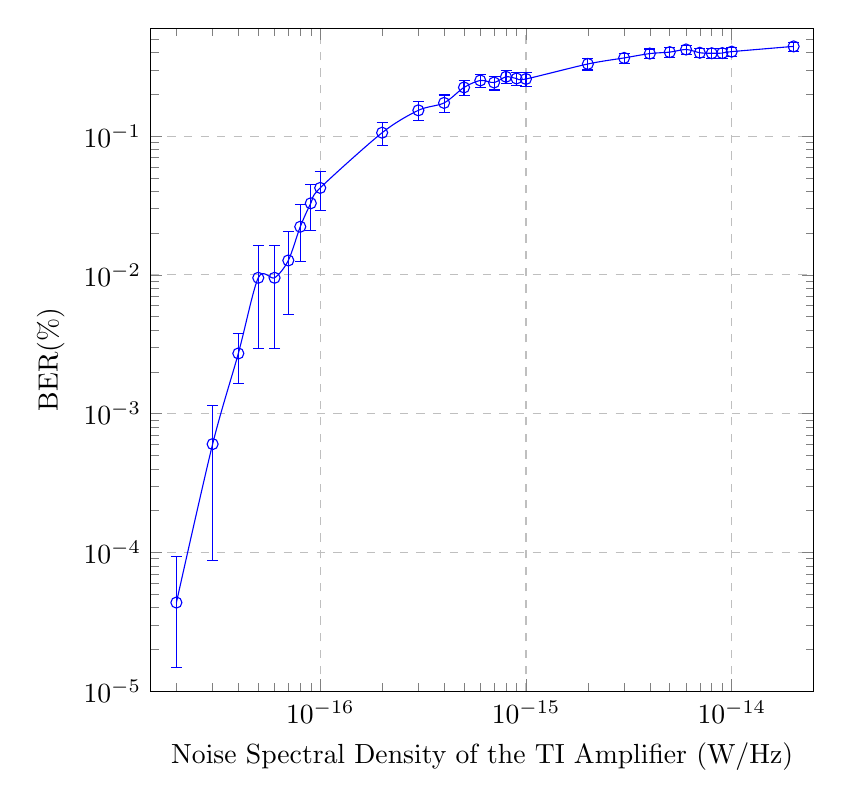
\begin{tikzpicture}
        \begin{axis}[
            height=10cm,
            width=10cm,
            xlabel=Noise Spectral Density of the TI Amplifier (W/Hz),
            ylabel=BER(\%),
            ymin=1e-5, ymax=0.6,
            xmin=1.5e-17, xmax=2.5e-14,
            ymode=log,
            xmode=log,
            ymajorgrids=true,
            xmajorgrids=true,
            grid style=dashed,
        ]
        \addplot[
            samples y=0,
            smooth,
            mark=o,
            blue,
            error bars/.cd, y dir=both, y explicit,
        ] plot coordinates {
            (2e-17,4.34783e-05) +=(0,4.9852e-05) -=(0,2.86804e-05)
            (3e-17,0.000603379) +=(0,0.000549511) -=(0,0.0005163459)
            (4e-17,0.00271521) +=(0,0.00108902) -=(0,0.00105709)
            (5e-17,0.0095339) +=(0,0.0068759) -=(0,0.00658128)
            (6e-17,0.0095339) +=(0,0.0068759) -=(0,0.00658128)
            (7e-17,0.0127119) +=(0,0.0078136) -=(0,0.00753854)
            (8e-17,0.0222458) +=(0,0.010046) -=(0,0.0098294)
            (9e-17,0.032839) +=(0,0.0119741) -=(0,0.0118224)
            (1e-16,0.0423729) +=(0,0.0134263) -=(0,0.0133331)
            (2e-16,0.105932) +=(0,0.020013) -=(0,0.0203095)
            (3e-16,0.153602) +=(0,0.023236) -=(0,0.023825)
            (4e-16,0.173729) +=(0,0.024342) -=(0,0.025055)
            (5e-16,0.224576) +=(0,0.026638) -=(0,0.027662)
            (6e-16,0.252119) +=(0,0.027633) -=(0,0.028827)
            (7e-16,0.243644) +=(0,0.027344) -=(0,0.028484)
            (8e-16,0.268008) +=(0,0.02814) -=(0,0.029429)
            (9e-16,0.260593) +=(0,0.027909) -=(0,0.029154)
            (1e-15,0.258475) +=(0,0.027841) -=(0,0.029074)
            (2e-15,0.331568) +=(0,0.029721) -=(0,0.031401)
            (3e-15,0.366525) +=(0,0.030321) -=(0,0.032215)
            (4e-15,0.394068) +=(0,0.030669) -=(0,0.032733)
            (5e-15,0.403602) +=(0,0.030766) -=(0,0.032888)
            (6e-15,0.42161) +=(0,0.030915) -=(0,0.033147)
            (7e-15,0.399364) +=(0,0.030725) -=(0,0.03282)
            (8e-15,0.396186) +=(0,0.030693) -=(0,0.032768)
            (9e-15,0.397246) +=(0,0.030703) -=(0,0.032786)
            (1e-14,0.40678) +=(0,0.030795) -=(0,0.032937)
            (2e-14,0.443856) +=(0,0.031039) -=(0,0.033408)

        };
        \end{axis}
    \end{tikzpicture}
\end{center}
We can observe that the BER decreases at an enlarging rate, as we augment the spectral density of the noise on the TI Amplifier. Giving us an estimate of the sensitivity of the receiver to thermal noise.


\begin{itemize}
    \item[--] Impact of the bandwidth of the TI Amplifier:
\end{itemize}
On the following graph we can see the impact of the bandwith of the electrical amplifier on the BER.\\
For the horizontal axes the used metric will be the ratio between the signal bandwidth and the TI Amplifier bandwidth, to better understand how these to relate, and the minimum requirements for a well suited electrical amplifier.\\
For the test, thermal noise will also be inserted, to also evaluate the impact of a too broad bandwidth.


        \begin{center}
        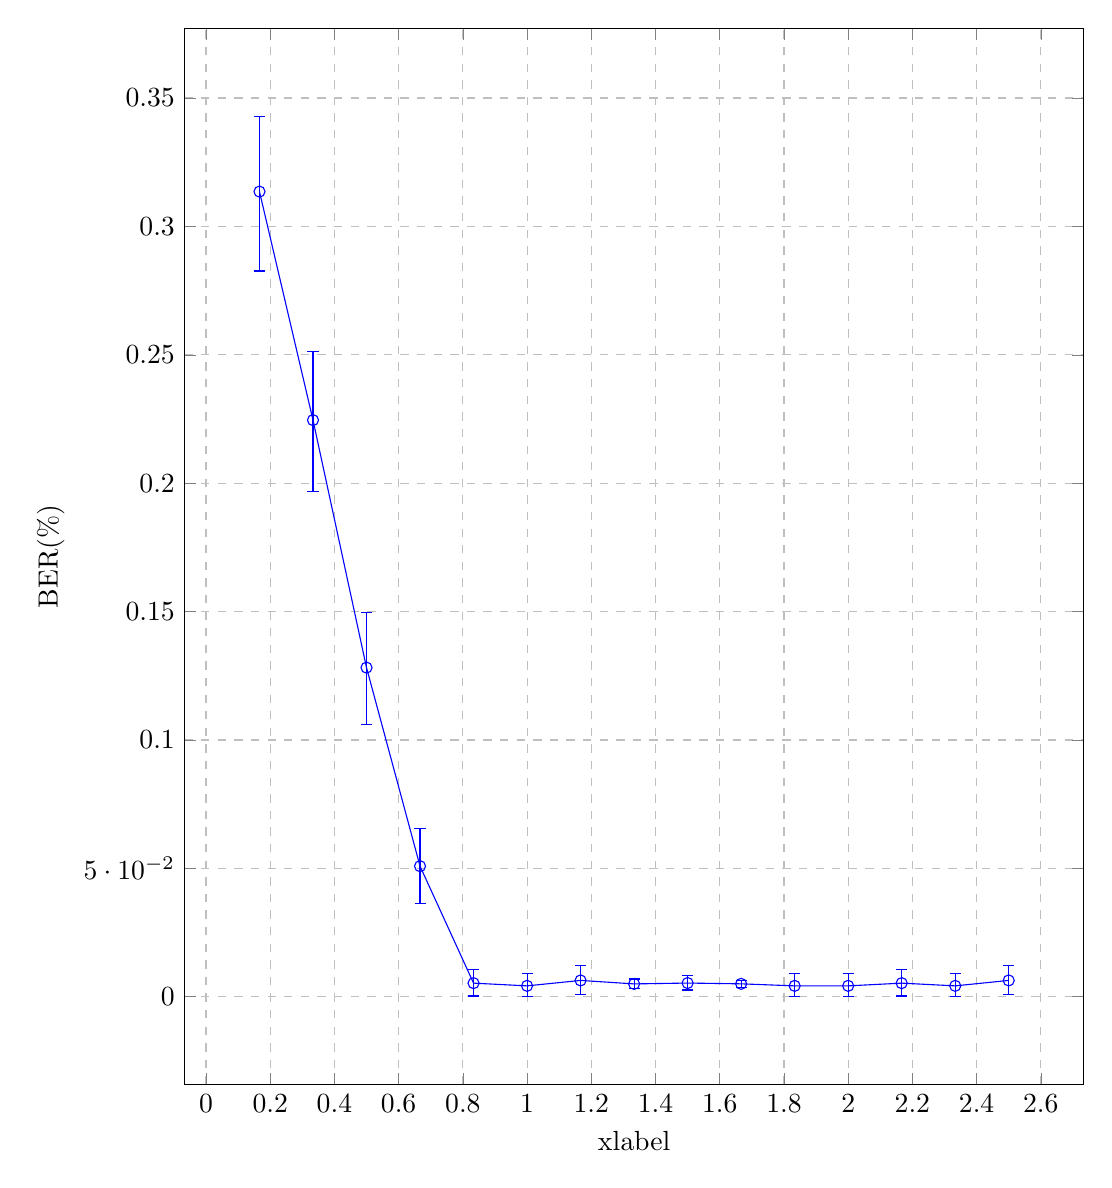
\begin{tikzpicture}
            \begin{axis}[
                height=15cm,
                width=13cm,
                xlabel=xlabel=Signal BW/TI Amplifier BW,,
                ylabel=BER(\%),
                %ymode=log,
                ymajorgrids=true,
                xmajorgrids=true,
                grid style=dashed,
            ]
            \addplot[
                samples y=0,
                %smooth,
                mark=o,
                blue,
                error bars/.cd, y dir=both, y explicit,
            ] plot coordinates {
                (0.166666666667,0.313559) +=(0,0.029341) -=(0,0.03091)
(0.333333333333,0.224576) +=(0,0.026638) -=(0,0.027662)
(0.5,0.128178) +=(0,0.021638) -=(0,0.022071)
(0.666666666667,0.0508475) +=(0,0.0145644) -=(0,0.0145231)
(0.833333333333,0.00529661) +=(0,0.00532029) -=(0,0.004999633)
(1.0,0.00423729) +=(0,0.00483688) -=(0,0.0042372899)
(1.16666666667,0.00635593) +=(0,0.00575627) -=(0,0.005442116)
(1.33333333333,0.005) +=(0,0.00192767) -=(0,0.00187519)
(1.5,0.00533333) +=(0,0.00282339) -=(0,0.00272256)
(1.66666666667,0.00502816) +=(0,0.00145578) -=(0,0.00142519)
(1.83333333333,0.00423729) +=(0,0.00483688) -=(0,0.0042372899)
(2.0,0.00423729) +=(0,0.00483688) -=(0,0.0042372899)
(2.16666666667,0.00529661) +=(0,0.00532029) -=(0,0.004999633)
(2.33333333333,0.00423729) +=(0,0.00483688) -=(0,0.0042372899)
(2.5,0.00635593) +=(0,0.00575627) -=(0,0.005442116)

            };
            \end{axis}
        \end{tikzpicture}
        \end{center}
        We can see that, on the simulator, the bandwidth of the TI Amplifier only has a significant effect when it is smaller than 80\% of the transmitted signal bandwidth. For higher bandwidths of the TI Amplifier (higher than the signal bandwidth) the simulator demonstrates no increase in the BER.



\subsection*{Functional description}

This block has an input of two optical signals, the received signal from the transmission channel and the signal from the local oscillator. These signals pass through a set of blocks, as it can be seen in figure\ref{fig:homodyneRx_blocks}, and then it outputs one binary signal that corresponds to the decoded information transmitted in the input signal from the transmission channel. \\
With this block we needn't to manually make all the connections between the different blocks needed to implement an optical receiver. All we need to do is create an instance of the block and only modify the parameters whose default values are not in accordance with our needs. All the methods available to do so have already been presented above.\\
It is a super block of higher complexity than the M-QAM Transmitter, making it harder to give a general overview of the signal flow, thus it is important to emphasize that, for any more specific doubts the documentation of the singular blocks should be addressed.
\begin{figure}[H]
	\centering \includegraphics[width=\textwidth]{../lib/m_qam_receiver/figures/simulation_rx.pdf}
	\caption{Schematic representation of the block homodyne
	receiver.}\label{fig:homodyneRx_blocks}
\end{figure}
The block Optical hybrid alongside with the photodetectors mix the oscillator signal with the input signal in order to convert a complex optical signal into two real electrical signals, these represent the in-phase and the quadrature components of the received signal.\\
We are now in the electrical domain and the signals are a function of the current in the photodetectors, but still working with very low amplitudes, thus we need to have an electrical transimpedance amplifier, that will increase the signal power. Then, noise is added to simulate thermal noise present in all electronics.\\
After having strong electrical signals, we need to sample them, for them to be processed by a digital signal processor.\\
Finally, the in-phase and quadrature signals, discrete in time but continuous in amplitude, are processed by a decoder, which translates pairs of amplitudes to a sequence of binary digits, using the maximum likelihood approach.


\subsection*{Open issues}
\begin{itemize}
  \item[--] The decoder only works for constellations in which all points have the same distance from the origin (example: QPSK). This is due to the fact that the decoder only takes into consideration which point of the constellation is closer to the received coordinates, but not the amplitude of the received signal. This means the decoder doesn't work properly for 16-QAM signals, making in impossible to analyse BER for cases that don't comply with the condition of all points being at the same distance from the origin;
  \item[--] The formula that is responsible for inserting the effect of the quantum noise on the photodetectors seems po be wrong, since the shot noise power is always much smaller than the signal power, even for values of 100dBm on the receiver's local oscillator;
  \item[--] There are a lot of parameters from the blocks included in the Receiver super block that can't be acessed/modified through methods of the Receiver, making it hard to configure the various parameters available for each block that constitutes the Receiver block.
\end{itemize}
\subsection*{Future improvements}
\begin{itemize}
  \item[--] Besides the binary signal, there could be an additional output signal that would easily allow us to observe the received constellation with the noise added by the receiver block;
  \item[--] Correction of the several issues.
\end{itemize}

